\documentclass[11pt,a4paper]{article}
\usepackage{amsmath,amssymb,amsfonts,bm}
\usepackage{tikz}
\usetikzlibrary{knots, hobby, calc, intersections, decorations.pathreplacing, decorations.markings, shapes.geometric, spath3}

% ==============================================================================
%  SST RENDER ENGINE: Twisted Dual-Strand Logic
% ==============================================================================

% -- Configuration --
\def\Wth{2.5pt}          % Strand width
\def\Core{white}         % Gap color (background color)
\def\Mask{5.0pt}         % Mask width for overlap
\def\ClrA{black!60!black}      % Strand A Color (Shadow)
\def\ClrB{red!70!black}  % Strand B Color (Main)
\def\Samples{400}        % Resolution

% -- Strand Style --
\tikzset{
    fat strand/.style={
        draw=#1, line width=\Wth,
        double=\Core, double distance=1.2*\Wth,
        line cap=round, line join=round
    }
}

% -- Coordinate Generator --
% #1: Path Definition, #2: Samples, #3: Amp, #4: Turns, #5: StrandName(A/B)
\newcommand{\MakeStrandCoords}[5]{%
    \pgfmathtruncatemacro{\Ns}{#2}
    \def\Phase{0}\ifx#5B\def\Phase{0.5}\fi
    \foreach \i in {0,...,\Ns}{%
        \pgfmathsetmacro{\s}{\i/\Ns}%
        \pgfmathsetmacro{\y}{#3*sin(360*(#4*\s + \Phase))}%
        \path[postaction={decorate, decoration={markings,
        mark=at position \s with {\coordinate (#5\i) at (0,\y);}}}] #1;%
    }%
}

% -- Segment Drawer --
\newcommand{\drawSeg}[4]{% #1:Name, #2:Index, #3:Color, #4:Over(0/1)
    \ifnum#4=1
    \draw[preaction={draw=\Core, line width=\Mask}, fat strand=#3]
    (#1#2) .. (#1\the\numexpr#2+1\relax);
    \else
        \draw[fat strand=#3]
        (#1#2) .. (#1\the\numexpr#2+1\relax);
    \fi
}

% -- Main Render Command --
    % #1: Path Macro (e.g., \KPATH), #2: Turns, #3: Amplitude
    \newcommand{\RenderTwist}[3]{
    \MakeStrandCoords{#1}{\Samples}{#3}{#2}{A}
    \MakeStrandCoords{#1}{\Samples}{#3}{#2}{B}
    \pgfmathtruncatemacro{\Last}{\Samples-1}
    \foreach \k in {0,...,\Last}{
        \pgfmathsetmacro{\s}{\k/\Samples}
        % Twist logic: swaps A/B depth based on sine phase
        \pgfmathtruncatemacro{\blk}{floor(2*#2*\s + 0.5)}
        \ifodd\blk
        \drawSeg{A}{\k}{\ClrA}{0}
        \drawSeg{B}{\k}{\ClrB}{1}
        \else
            \drawSeg{B}{\k}{\ClrB}{0}
            \drawSeg{A}{\k}{\ClrA}{1}
        \fi
    }
}

% -- Classic knot diagram (tikz-knot library, over/under crossings) --
% Zelfde aanroep als RenderTwist: wissel alleen de commandonaam.
% Optioneel getal aan het EINDE: \RenderStrand{\KPATH}{25}{0.13}[20] → flip 2,4,...,20.
\makeatletter
\def\RenderStrand@empty{}
\newcommand{\RenderStrand}[3]{%
    \@ifnextchar[{\RenderStrand@readopt{#1}{#2}{#3}}{\RenderStrand@doopt{#1}{#2}{#3}{}}%
}
\def\RenderStrand@readopt#1#2#3[#4]{%
    \RenderStrand@doopt{#1}{#2}{#3}{#4}%
}
\newcommand{\RenderStrand@doopt}[4]{%
    \if\relax\detokenize{#4}\relax
        \begin{knot}[
            consider self intersections,
            clip width=5pt, clip radius=3pt,
            ignore endpoint intersections=false
        ]
        \strand #1;
        \end{knot}%
    \else
        \def\RenderStrand@list{\RenderStrand@empty}%
        \foreach \i in {2,4,...,#4} {%
            \xdef\RenderStrand@list{\ifx\RenderStrand@list\RenderStrand@empty\i\else\RenderStrand@list,\i\fi}%
        }%
        \begin{knot}[
            consider self intersections,
            clip width=5pt, clip radius=3pt,
            ignore endpoint intersections=false,
            flip crossing/.list={\RenderStrand@list}
        ]
        \strand #1;
        \end{knot}%
    \fi
}
\makeatother

% -- Debug/Guide Points (Optional) --
\newcommand{\SSTGuidesPoints}[2]{
    \foreach \i in {1,...,#2}{
        \fill[blue] (P\i) circle (1.5pt);
        \node[blue,font=\tiny,above right] at (P\i) {\i};
    }
}

\begin{document}

% ==============================================================================
%  1. THE UNKNOT (0_1)
%     "The Vacuum State / Trivial Topology"
% ==============================================================================
    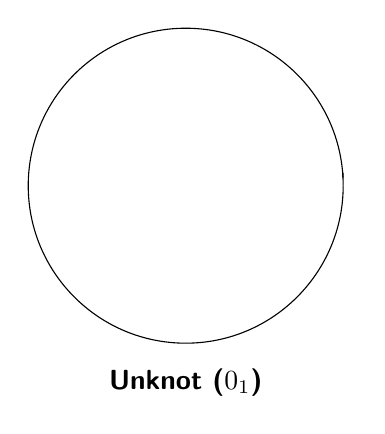
\begin{tikzpicture}[use Hobby shortcut]
        \def\KPATH{(0,0) circle (2cm)}
        \RenderStrand{\KPATH}{6}{0.15} % 6 Turns
        \node[font=\bfseries\sffamily] at (0,-2.5) {Unknot ($0_1$)};
    \end{tikzpicture}

% ==============================================================================
%  2. TREFOIL (3_1)
%     "Fundamental Fermion Generation"
% ==============================================================================
    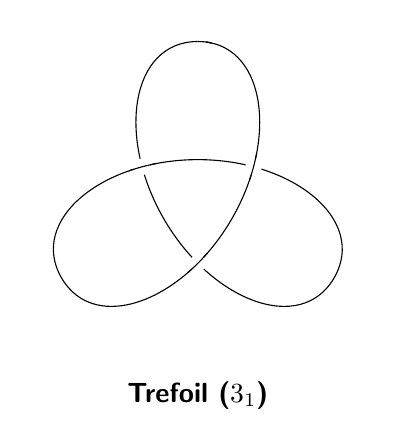
\begin{tikzpicture}[use Hobby shortcut]
        % Explicit Coordinates derived from parametric: R_outer=2.0, R_inner=-0.5
        \coordinate (P1) at (0, 2);             % Start/Top Lobe
        \coordinate (P2) at (0.433, -0.25);     % Inner Crossing 1
        \coordinate (P3) at (-1.732, -1);       % Left Lobe
        \coordinate (P4) at (0, 0.5);           % Top Inner Crossing
        \coordinate (P5) at (1.732, -1);        % Right Lobe
        \coordinate (P6) at (-0.433, -0.25);    % Inner Crossing 2
        \coordinate (P7) at (0, 2);             % Close = P1

        \def\KPATH{
            ([closed] P1)..(P2)..(P3)..(P4)..(P5)..(P6)..(P7)
        }

        \RenderStrand{\KPATH}{12}{0.15}
        \node[font=\bfseries\sffamily] at (0,-2.5) {Trefoil ($3_1$)};
    \end{tikzpicture}

% ==============================================================================
%  3. CINQUEFOIL (5_1)
%     "Higher Generation Resonance"
% ==============================================================================
    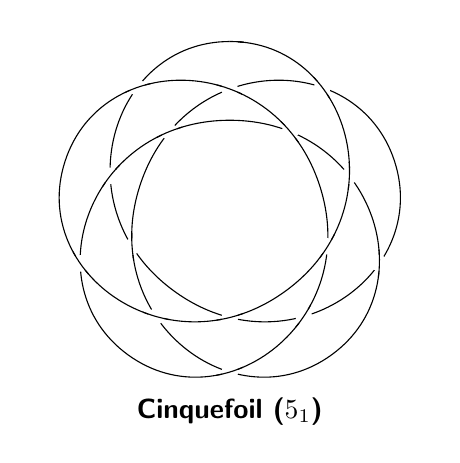
\begin{tikzpicture}[use Hobby shortcut]
        % Explicit Coordinates: R_outer=2.2, R_inner=-1.2 (Star Polygon)
        \coordinate (P1)  at (0, 2.2);            % Top Lobe
        \coordinate (P2)  at (0.705, -0.971);     % Inner 1
        \coordinate (P3)  at (-2.092, 0.680);     % Lobe 2
        \coordinate (P4)  at (1.141, 0.371);      % Inner 2
        \coordinate (P5)  at (-1.293, -1.779);    % Lobe 3
        \coordinate (P6)  at (0, 1.200);          % Inner 3 (Top Crossing)
        \coordinate (P7)  at (1.293, -1.779);     % Lobe 4
        \coordinate (P8)  at (-1.141, 0.371);     % Inner 4
        \coordinate (P9)  at (2.092, 0.680);      % Lobe 5
        \coordinate (P10) at (-0.705, -0.971);    % Inner 5
        \coordinate (P11) at (0, 2.2);            % Close = P1

        \def\KPATH{
            ([closed] P1)..(P2)..(P3)..(P4)..(P5)..(P6)..(P7)..(P8)..(P9)..(P10)..(P11)
        }

        \RenderStrand{\KPATH}{18}{0.15}
        \node[font=\bfseries\sffamily] at (0,-2.5) {Cinquefoil ($5_1$)};
    \end{tikzpicture}

% ==============================================================================
%  4. SEPTAFOIL (7_1)
%     "Hypothetical High-Energy State"
% ==============================================================================
    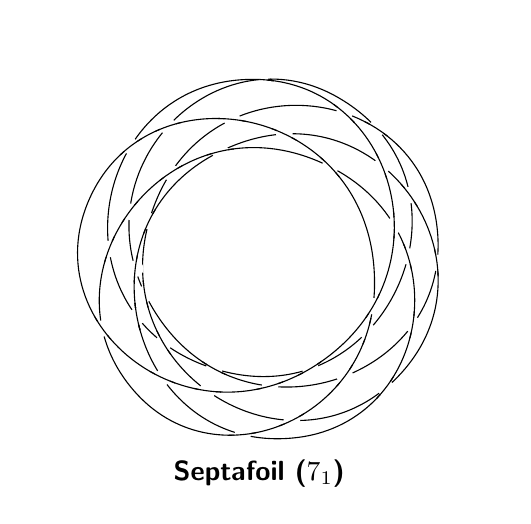
\begin{tikzpicture}[use Hobby shortcut]
        % Explicit Coordinates: R_outer=2.3, R_inner=-1.5
        \coordinate (P1)  at (0, 2.3);             % Lobe 1 (Top)
        \coordinate (P2)  at (0.871, -1.222);      % Inner 1
        \coordinate (P3)  at (-2.189, 0.706);      % Lobe 2
        \coordinate (P4)  at (1.464, -0.328);      % Inner 2
        \coordinate (P5)  at (-1.551, -1.698);     % Lobe 3
        \coordinate (P6)  at (0.932, 1.175);       % Inner 3
        \coordinate (P7)  at (0.505, -2.244);      % Lobe 4
        \coordinate (P8)  at (-0.312, 1.467);      % Inner 4
        \coordinate (P9)  at (1.795, -1.438);      % Lobe 5
        \coordinate (P10) at (-1.353, 0.647);      % Inner 5
        \coordinate (P11) at (2.254, 0.457);       % Lobe 6
        \coordinate (P12) at (-1.419, -0.486);     % Inner 6
        \coordinate (P13) at (1.009, 2.067);       % Lobe 7
        \coordinate (P14) at (-0.685, -1.334);     % Inner 7
        \coordinate (P15) at (0, 2.3);             % Close = P1

        \def\KPATH{
            ([closed] P1)..(P2)..(P3)..(P4)..(P5)..(P6)..(P7)..(P8)
            ..(P9)..(P10)..(P11)..(P12)..(P13)..(P14)..(P15)
        }

        \RenderStrand{\KPATH}{24}{0.12}
        \node[font=\bfseries\sffamily] at (0,-2.7) {Septafoil ($7_1$)};
    \end{tikzpicture}
% ==============================================================================
%  5. (5_2)
%     SST Specific Geometry
% ==============================================================================
    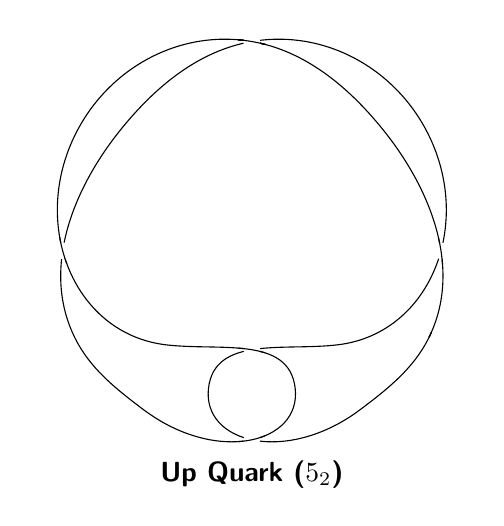
\begin{tikzpicture}[use Hobby shortcut, scale=1.1]
        % Explicit Coordinates from SST Canon
        \coordinate (P1) at (2, -1.5);
        \coordinate (P2) at (1.5, 1);
        \coordinate (P3) at (0, 2);
        \coordinate (P4) at (-2, 1);
        \coordinate (P5) at (-1, -1.5);
        \coordinate (P6) at (0.5, -2);
        \coordinate (P7) at (-1.25, -2.25);
        \coordinate (P8) at (-2, -1.5);
        \coordinate (P9) at (-1.5, 1);
        \coordinate (P10) at (0, 2);
        \coordinate (P11) at (2, 1);
        \coordinate (P12) at (1, -1.5);
        \coordinate (P13) at (-0.5, -2);
        \coordinate (P14) at (1.25, -2.25);
        \coordinate (P15) at (2, -1.5); % = P1

        \def\KPATH{
            ([closed] P1)..(P2)..(P3)..(P4)..(P5)..(P6)..(P7)..(P8)
            ..(P9)..(P10)..(P11)..(P12)..(P13)..(P14)..(P15)
        }

        \RenderStrand{\KPATH}{22}{0.13}
        \node[font=\bfseries\sffamily] at (0,-3.0) {Up Quark ($5_2$)};
    \end{tikzpicture}

% ==============================================================================
%  6. DOWN QUARK (6_1 - Stevedore)
%     SST Specific Geometry
% ==============================================================================
    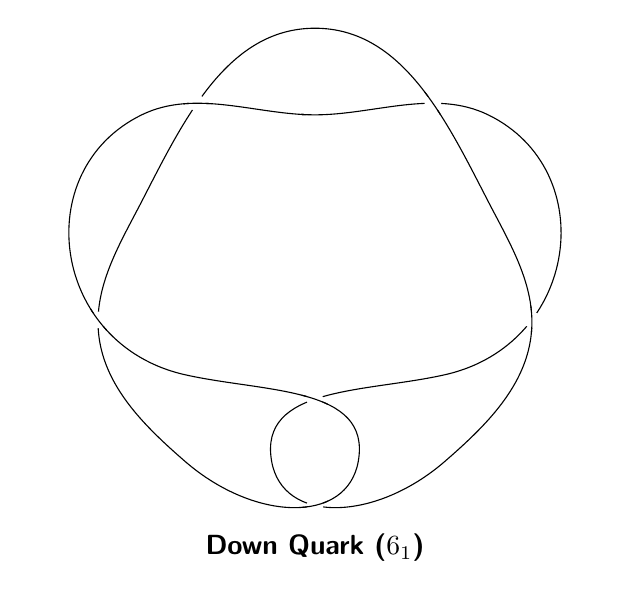
\begin{tikzpicture}[use Hobby shortcut, scale=1.1]
        % Explicit Coordinates from SST Canon
        \coordinate (P1)  at ( 0,  2);
        \coordinate (P2)  at (-2,  2);
        \coordinate (P3)  at (-1.5, -1);
        \coordinate (P4)  at ( 0.5, -2);
        \coordinate (P5)  at (-1.5,-2);
        \coordinate (P6)  at (-2.5,-0.5);
        \coordinate (P7)  at (-2, 1);
        \coordinate (P8)  at ( 0,  3);
        \coordinate (P9)  at ( 2, 1);
        \coordinate (P10) at ( 2.5,-0.5);
        \coordinate (P11) at ( 1.5,-2);
        \coordinate (P12) at (-0.5, -2);
        \coordinate (P13) at ( 1.5, -1);
        \coordinate (P14) at ( 2,  2);
        \coordinate (P15) at ( 0,  2); % = P1

        \def\KPATH{
            ([closed] P1)..(P2)..(P3)..(P4)..(P5)..(P6)..(P7)..(P8)
            ..(P9)..(P10)..(P11)..(P12)..(P13)..(P14)..(P15)
        }

        \RenderStrand{\KPATH}{25}{0.13}[20]
        \node[font=\bfseries\sffamily] at (0,-3.0) {Down Quark ($6_1$)};
    \end{tikzpicture}

    
    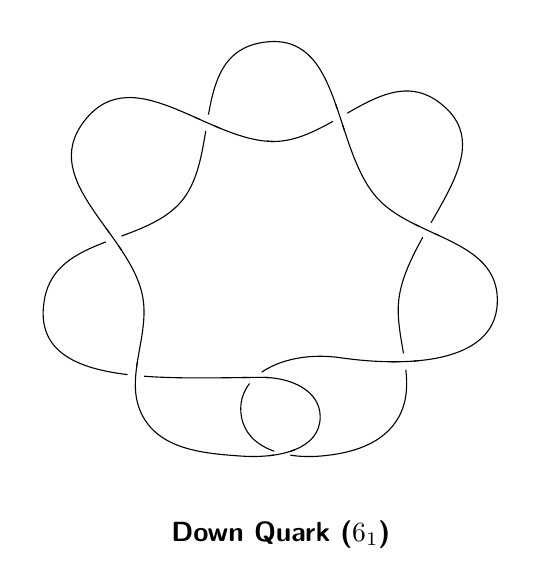
\begin{tikzpicture}[use Hobby shortcut]
    \coordinate (P1) at (0, 2);
    \coordinate (P2) at (-2.50, 2.25);
    \coordinate (P3) at (-1.75, 0);
    \coordinate (P4) at (-1.75, -1.50);
    \coordinate (P5) at (-0.50, -2);
    \coordinate (P6) at (0.50, -1.50);
    \coordinate (P7) at (-0.25, -1);
    \coordinate (P8) at (-3, 0);
    \coordinate (P9) at (-1.25, 1.25);
    \coordinate (P10) at (-0.25, 3.25);
    \coordinate (P11) at (1.25, 1.25);
    \coordinate (P12) at (2.75, 0);
    \coordinate (P13) at (0.75, -0.75);
    \coordinate (P14) at (-0.50, -1.50);
    \coordinate (P15) at (0.50, -2);
    \coordinate (P16) at (1.50, -1.50);
    \coordinate (P17) at (1.50, 0);
    \coordinate (P18) at (2, 2.50);

    \def\KPATH{
        ([closed] P1)..(P2)..(P3)..(P4)..(P5)..(P6)..(P7)..(P8)..(P9)..(P10)..(P11)..(P12)..(P13)..(P14)..(P15)..(P16)..(P17)..(P18)
    }
    % Kies één: twisted dual-strand of classic knot (zelfde aanroep, andere commandonaam).
    % Bij RenderStrand: optioneel getal = max crossing-index → flip 2,4,...,20 (bijv. 20 voor 6_1).
    % \RenderTwist{\KPATH}{25}{0.13}
    \RenderStrand{\KPATH}{25}{0.13}[20]
    \node[font=\bfseries\sffamily] at (0,-3.0) {Down Quark ($6_1$)};
    %\SSTGuidesPoints{P}{18}
    \end{tikzpicture}

    
    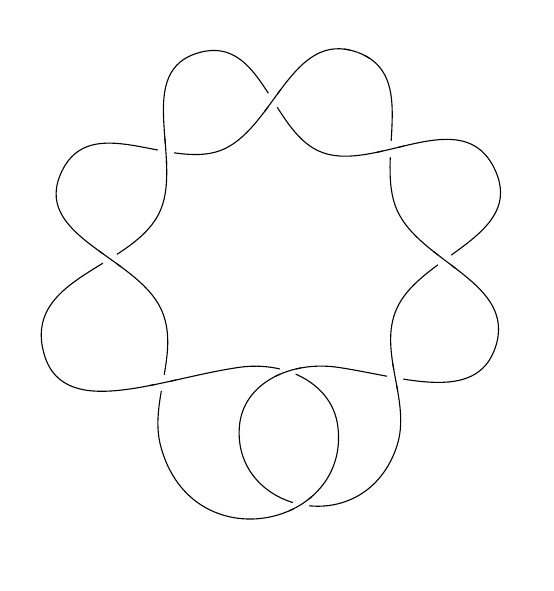
\begin{tikzpicture}[use Hobby shortcut]
    \coordinate (P1) at (0.75, 3.25);
    \coordinate (P2) at (-1, 2);
    \coordinate (P3) at (-3, 1.75);
    \coordinate (P4) at (-1.75, 0);
    \coordinate (P5) at (-1.75, -1.75);
    \coordinate (P6) at (0.50, -1.50);
    \coordinate (P7) at (-0.75, -0.75);
    \coordinate (P8) at (-3.25, -0.50);
    \coordinate (P9) at (-1.75, 1.25);
    \coordinate (P10) at (-1.25, 3.25);
    \coordinate (P11) at (0.25, 2);
    \coordinate (P12) at (2.50, 1.75);
    \coordinate (P13) at (1.25, 0);
    \coordinate (P14) at (1.25, -1.75);
    \coordinate (P15) at (-0.75, -1.50);
    \coordinate (P16) at (0.50, -0.75);
    \coordinate (P17) at (2.50, -0.50);
    \coordinate (P18) at (1.25, 1.25);

    \begin{knot}[
        consider self intersections,
        clip width=5pt, clip radius=3pt,
        ignore endpoint intersections=false,
        flip crossing/.list={2,4,6,8,10,12,14,16,18,20},
        % ----draft mode=crossings % uncomment to see numbers
    ]
    \strand
    ([closed] P1)..(P2)..(P3)..(P4)..(P5)..(P6)..(P7)..(P8)..(P9)..(P10)..(P11)..(P12)..(P13)..(P14)..(P15)..(P16)..(P17)..(P18);
    \end{knot}
    %\SSTGuidesPoints{P}{18}
    \end{tikzpicture}

    
    \begin{tikzpicture}[use Hobby shortcut]
    \coordinate (P1) at (0.25, 3.25);
    \coordinate (P2) at (-1.25, 2);
    \coordinate (P3) at (-3.25, 1.50);
    \coordinate (P4) at (-2.25, -0.50);
    \coordinate (P5) at (-2, -2.50);
    \coordinate (P6) at (0.25, -1.75);
    \coordinate (P7) at (2.25, -1.75);
    \coordinate (P8) at (1.75, 0);
    \coordinate (P9) at (2.25, 2.25);
    \coordinate (P10) at (0.25, 2.25);
    \coordinate (P11) at (-1.75, 3);
    \coordinate (P12) at (-2.25, 1);
    \coordinate (P13) at (-3.50, -0.75);
    \coordinate (P14) at (-1.50, -1.25);
    \coordinate (P15) at (0.75, -3);
    \coordinate (P16) at (1.25, -1);
    \coordinate (P17) at (3, 0.25);
    \coordinate (P18) at (1, 2);

    \begin{knot}[
        consider self intersections,
        clip width=5pt, clip radius=3pt,
        ignore endpoint intersections=false,
        flip crossing/.list={2,4,6,8,10,12,14,16,18,20},
        % ----draft mode=crossings % uncomment to see numbers
    ]
    \strand
    ([closed] P1)..(P2)..(P3)..(P4)..(P5)..(P6)..(P7)..(P8)..(P9)..(P10)..(P11)..(P12)..(P13)..(P14)..(P15)..(P16)..(P17)..(P18);
    \end{knot}
    %\SSTGuidesPoints{P}{18}
    \end{tikzpicture}

    
    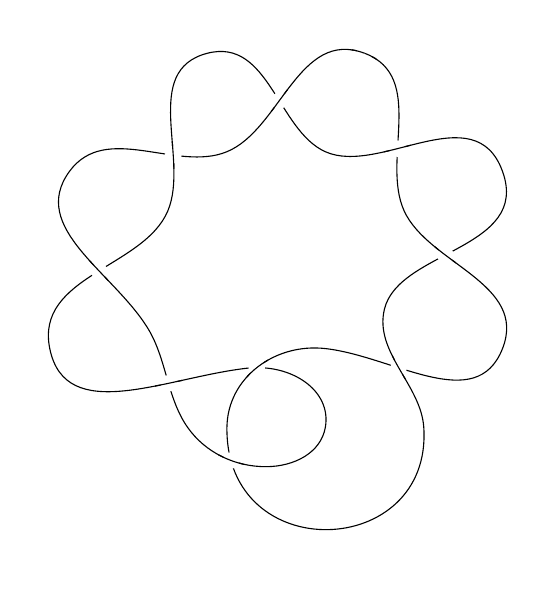
\begin{tikzpicture}[use Hobby shortcut]
    \coordinate (P1) at (0.75, 3.25);
    \coordinate (P2) at (-1, 2);
    \coordinate (P3) at (-3, 1.75);
    \coordinate (P4) at (-2, -0.25);
    \coordinate (P5) at (-1.50, -1.50);
    \coordinate (P6) at (-0.50, -2);
    \coordinate (P7) at (0.25, -1.50);
    \coordinate (P8) at (-0.75, -0.75);
    \coordinate (P9) at (-3.25, -0.50);
    \coordinate (P10) at (-1.75, 1.25);
    \coordinate (P11) at (-1.25, 3.25);
    \coordinate (P12) at (0.25, 2);
    \coordinate (P13) at (2.50, 1.75);
    \coordinate (P14) at (1, 0);
    \coordinate (P15) at (1.50, -1.50);
    \coordinate (P16) at (-1, -1.50);
    \coordinate (P17) at (0.25, -0.50);
    \coordinate (P18) at (2.50, -0.50);
    \coordinate (P19) at (1.25, 1.25);

    \begin{knot}[
        consider self intersections,
        clip width=5pt, clip radius=3pt,
        ignore endpoint intersections=false,
        flip crossing/.list={2,4,6,8,10,12,14,16,18,20},
        % ----draft mode=crossings % uncomment to see numbers
    ]
    \strand
    ([closed] P1)..(P2)..(P3)..(P4)..(P5)..(P6)..(P7)..(P8)..(P9)..(P10)..(P11)..(P12)..(P13)..(P14)..(P15)..(P16)..(P17)..(P18)..(P19);
    \end{knot}
    %\SSTGuidesPoints{P}{19}
    \end{tikzpicture}

    
    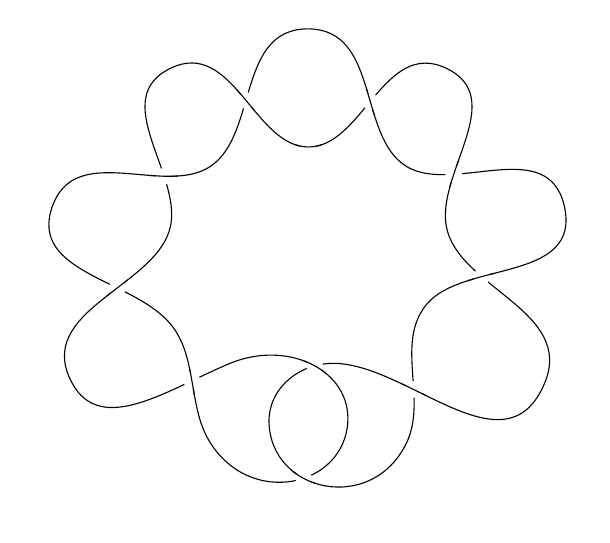
\begin{tikzpicture}[use Hobby shortcut]
    \coordinate (P1) at (0, 2);
    \coordinate (P2) at (-1.75, 3);
    \coordinate (P3) at (-1.75, 1);
    \coordinate (P4) at (-3, -1);
    \coordinate (P5) at (-1, -0.75);
    \coordinate (P6) at (0.50, -1.50);
    \coordinate (P7) at (-1.25, -1.75);
    \coordinate (P8) at (-1.75, -0.25);
    \coordinate (P9) at (-3.25, 1.25);
    \coordinate (P10) at (-1.25, 1.75);
    \coordinate (P11) at (0, 3.50);
    \coordinate (P12) at (1.25, 1.75);
    \coordinate (P13) at (3.25, 1.25);
    \coordinate (P14) at (1.50, 0);
    \coordinate (P15) at (1.25, -1.75);
    \coordinate (P16) at (-0.50, -1.50);
    \coordinate (P17) at (0.25, -0.75);
    \coordinate (P18) at (3, -1);
    \coordinate (P19) at (1.75, 1);
    \coordinate (P20) at (1.75, 3);

    \begin{knot}[
        consider self intersections,
        clip width=5pt, clip radius=3pt,
        ignore endpoint intersections=false,
        flip crossing/.list={2,4,6,8,10,12,14,16,18,20},
        % ----draft mode=crossings % uncomment to see numbers
    ]
    \strand
    ([closed] P1)..(P2)..(P3)..(P4)..(P5)..(P6)..(P7)..(P8)..(P9)..(P10)..(P11)..(P12)..(P13)..(P14)..(P15)..(P16)..(P17)..(P18)..(P19)..(P20);
    \end{knot}
    %\SSTGuidesPoints{P}{20}
    \end{tikzpicture}

    
\end{document}